\documentclass{article} % For LaTeX2e
\usepackage{nips14submit_e,times}
\usepackage{amsmath}
\usepackage{amsthm}
\usepackage{amssymb}
\usepackage{mathtools}
\usepackage{hyperref}
\usepackage{url}
\usepackage{algorithm}
\usepackage[noend]{algpseudocode}
%\documentstyle[nips14submit_09,times,art10]{article} % For LaTeX 2.09

\usepackage{bbm}
\usepackage{graphicx}
\usepackage{caption}
\usepackage{subcaption}
\usepackage{MnSymbol}

\def\eQb#1\eQe{\begin{eqnarray*}#1\end{eqnarray*}}
\def\eQnb#1\eQne{\begin{eqnarray}#1\end{eqnarray}}
\providecommand{\e}[1]{\ensuremath{\times 10^{#1}}}
\providecommand{\pb}[0]{\pagebreak}
\DeclarePairedDelimiter\ceil{\lceil}{\rceil}
\DeclarePairedDelimiter\floor{\lfloor}{\rfloor}

\newcommand{\E}{\mathrm{E}}
\newcommand{\Var}{\mathrm{Var}}
\newcommand{\Cov}{\mathrm{Cov}}
\newcommand\eqD{\stackrel{\mathclap{\normalfont\mbox{d}}}{=}}

\def\Qb#1\Qe{\begin{question}#1\end{question}}
\def\Sb#1\Se{\begin{solution}#1\end{solution}}

\newenvironment{claim}[1]{\par\noindent\underline{Claim:}\space#1}{}
\newtheoremstyle{quest}{\topsep}{\topsep}{}{}{\bfseries}{}{ }{\thmname{#1}\thmnote{ #3}.}
\theoremstyle{quest}
\newtheorem*{definition}{Definition}
\newtheorem*{theorem}{Theorem}
\newtheorem*{lemma}{Lemma}
\newtheorem*{question}{Question}
\newtheorem*{preposition}{Preposition}
\newtheorem*{exercise}{Exercise}
\newtheorem*{challengeproblem}{Challenge Problem}
\newtheorem*{solution}{Solution}
\newtheorem*{remark}{Remark}
\usepackage{verbatimbox}
\usepackage{listings}
\usepackage{mathrsfs}
\title{ProbLimI: \\
Problem Set VI}


\author{
Youngduck Choi \\
CIMS \\
New York University\\
\texttt{yc1104@nyu.edu} \\
}


% The \author macro works with any number of authors. There are two commands
% used to separate the names and addresses of multiple authors: \And and \AND.
%
% Using \And between authors leaves it to \LaTeX{} to determine where to break
% the lines. Using \AND forces a linebreak at that point. So, if \LaTeX{}
% puts 3 of 4 authors names on the first line, and the last on the second
% line, try using \AND instead of \And before the third author name.

\newcommand{\fix}{\marginpar{FIX}}
\newcommand{\new}{\marginpar{NEW}}

\nipsfinalcopy % Uncomment for camera-ready version

\begin{document}


\maketitle

\begin{abstract}
This work contains solutions to the exercises of the problem set V. The
chosen problems are 1,2, and 3.
\end{abstract}

\bigskip

\begin{question}[1]
\hfill
\begin{figure}[h!]
  \centering
    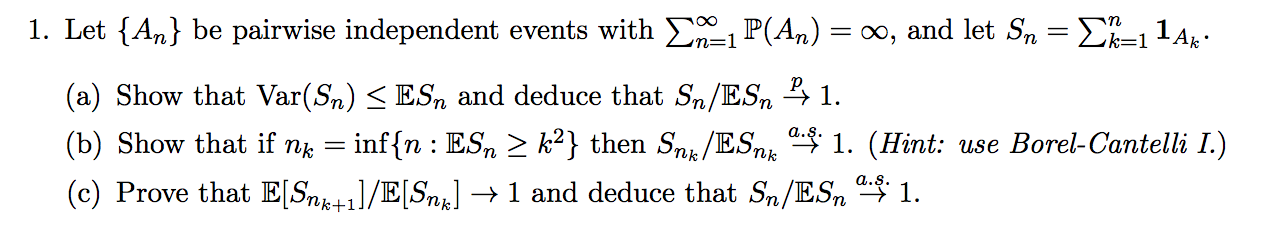
\includegraphics[width=0.7\textwidth]{prob-e6-p1.png}
\end{figure}
\end{question}
\begin{solution} \hfill \\
Observe that 
\eQb
\sum_{k=1}^{n} \mathbb{P}(A_k) &=& \mathbb{E}[S_n]  
\eQe 
for any $n \in \mathbb{N}$. As the LHS tends to $\infty$ as $n \to \infty$, 
we can choose $N$ large enough such that
$\mathbb{E}[S_n] > 0$ for all $n \geq N$. We relabel the indices to start from
$N$ so that the random variables $\{ \dfrac{S_n}{\mathbb{E}[S_n]}\}$ are well-defined
for the problem. 

\bigskip

\textbf{(i)} By independence,
\eQb
\Var(S_n) &=& \sum_{k=1}^{n} \Var(1_{A_k}) = \sum_{k=1}^{n} \mathbb{E}[1_{A_k}^2]
- \mathbb{E}[1_{A_k}]^2 = \sum_{k=1}^{n} \mathbb{P}(1_{A_k}) - 
\mathbb{P}(1_{A_k})^2 \\
&\leq& \sum_{k=1}^{n} \mathbb{P}(1_{A_k}) = \mathbb{E}[S_n]  
\eQe
for each $n \geq 1$. Now, we prove the claimed convergence in probability.
Let $\epsilon > 0$. By Chebyshev's inequality and the above result,
\eQb
\mathbb{P}(|\dfrac{S_n}{\mathbb{E}[S_n]} -1 | > \epsilon) &=&
\mathbb{P}(|S_n - \mathbb{E}[S_n]| > \epsilon \mathbb{E}[S_n]) \\
&\leq& \dfrac{\Var(S_n)}{\epsilon^2  \mathbb{E}[S_n]^2} \leq \dfrac{1}{\epsilon^2
\mathbb{E}[S_n]} 
\eQe
for any $ n \in \mathbb{N}$. Therefore, taking $n \to \infty$, 
\eQb
\lim_{n \to \infty} \mathbb{P}(|\dfrac{S_n}{\E[S_n]} - 1| > \epsilon) &=& 0.
\eQe
Since $\epsilon > 0$ was arbitrary, $\dfrac{S_n}{\E[S_n]} \to 1$ in probability. 

\bigskip

\textbf{(ii)} As $\mathbb{E}[S_n]$ tends to $\infty$ as $n \to \infty$, 
we can find a subsequence with the given property. 
Let $\epsilon > 0$. By the same argument as above, and the property
of the chosen subsequence, 
\eQb
\mathbb{P}(|\dfrac{S_n}{\mathbb{E}[S_n]} - 1| > \epsilon) &\leq& 
\dfrac{1}{\epsilon^2 \mathbb{E}[S_n]} \leq \dfrac{1}{\epsilon^2 k^2}  
\eQe
for all $k \in \mathbb{N}$, which implies
\eQb
\sum_{k=}^{\infty} \mathbb{P}(|\dfrac{S_{n_k}}{\mathbb{E}[S_{n_k}]} - 1| > 
\epsilon) < \infty.
\eQe
By Borel-Cantelli I, 
\eQb
\mathbb{P}(|\dfrac{S_{n_k}}{\mathbb{E}[S_{n_k}]} - 1| > \epsilon \>\>\>\> i.o) &=& 0
\eQe
Since $\epsilon > 0$ was arbitrary,
\eQb
\dfrac{S_{n_k}}{\mathbb{E}[S_{n_k}]} &\to& 1 \>\>\> \text{almost surely}.
\eQe

\end{solution}

\newpage

\begin{question}[2]
\hfill
\begin{figure}[h!]
  \centering
    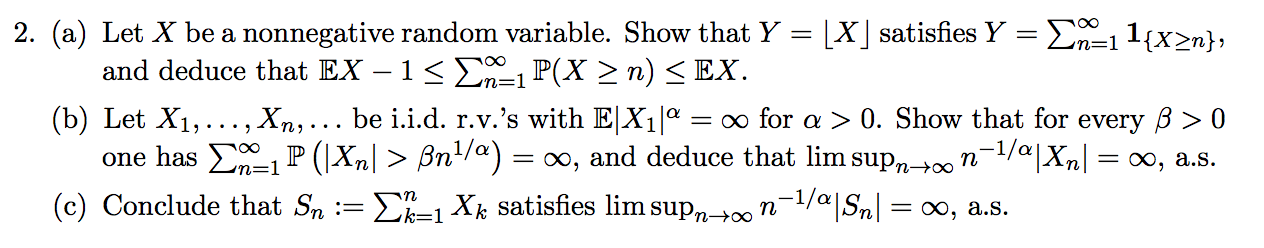
\includegraphics[width=0.7\textwidth]{prob-e6-p2.png}
\end{figure}
\end{question}
\begin{solution} \hfill \\
\end{solution}

\newpage

\begin{question}[3]
\hfill
\begin{figure}[h!]
  \centering
    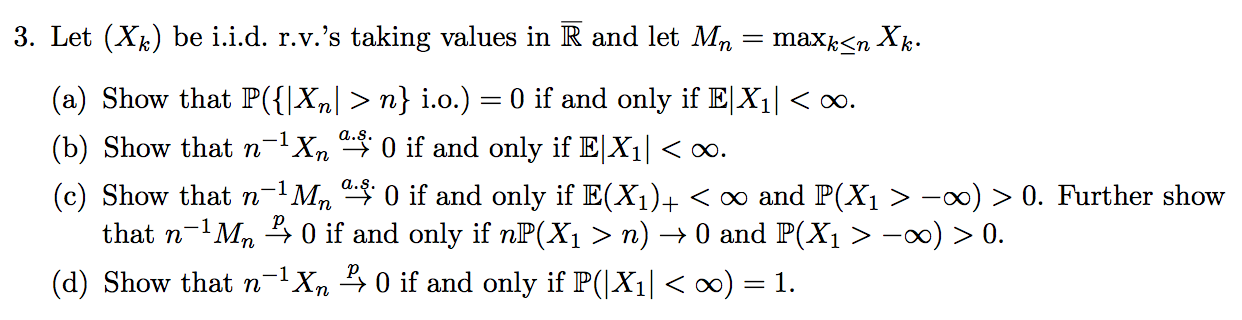
\includegraphics[width=0.7\textwidth]{prob-e6-p3.png}
\end{figure}
\end{question}
\begin{solution} \hfill \\
\end{solution}

\newpage

\begin{question}[4]
\hfill
\begin{figure}[h!]
  \centering
    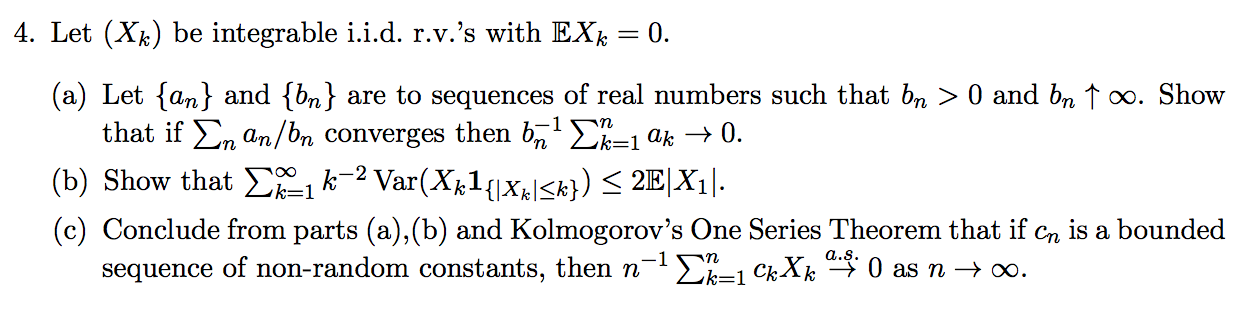
\includegraphics[width=0.7\textwidth]{prob-e6-p4.png}
\end{figure}
\end{question}
\begin{solution} \hfill \\
\end{solution}
\end{document}
